\chapter{METODOLOGIA E CRONOGRAMA}
\label{cap:metodologia}

Este capítulo descreve a abordagem metodológica adotada, que combina uma Revisão Sistemática da Literatura (detalhada no Apêndice A) e um survey exploratório (resultados completos no Apêndice B) com a metodologia de Design Science Research para o desenvolvimento do artefato proposto. 

% --- SEÇÃO PRINCIPAL SOBRE METODOLOGIA ---
\section{Abordagem Metodológica}
\label{sec:abordagem-metodologica}
Este trabalho adota uma abordagem metodológica mista, combinando métodos de pesquisa bibliográfica e empírica para garantir uma fundamentação sólida tanto no estado da arte quanto no contexto prático do problema investigado.

\subsection{Revisão Sistemática da Literatura}
\label{subsec:revisao-sistematica}

Para mapear o estado da arte sobre o uso de logs no ensino de programação, foi conduzida uma Revisão Sistemática da Literatura (RSL) seguindo as diretrizes de \cite{kitchenham2004procedures} e o protocolo PRISMA \cite{page2021prisma}. A revisão, detalhada na Seção \ref{sec:identificacao-estudos}, foi realizada em cinco bases de dados acadêmicas e resultou na seleção de 17 estudos para análise qualitativa. O processo de seleção, ilustrado no fluxograma PRISMA (Figura \ref{fig:prisma_flowchart}), seguiu critérios rigorosos de inclusão e exclusão. O protocolo completo encontra-se no \textbf{Apêndice A}.

\subsection{Survey Exploratório}
\label{subsec:survey}

Complementarmente à RSL, foi realizado um survey com 14 participantes, docentes, mestrandos em computação e pesquisadores de computação em foco no ensino de programação com o objetivo de investigar o uso de ferramentas de capturas de logs e construção de avaliações quantitativas e desenvolvimento de dataset acadêmicos. O instrumento de coleta continha 10 questões abordando logs, uso de ferramentas e IDEs. As respostas completas do survey e a análise detalhada encontram-se no \textbf{Apêndice B}.

\subsection{Design Science Research}
\label{subsec:dsr}

Este trabalho adota a abordagem de Design Science Research (DSR), conforme proposto por \cite{peffers2007design} e \cite{hevner2004design}. O DSR é adequado para pesquisas que visam desenvolver e avaliar artefatos que resolvam problemas identificados em contextos organizacionais e educacionais.

O processo de DSR será executado em quatro atividades principais:

\subsubsection{Atividade 1: Identificação do Problema e Motivação}
\label{subsubsec:problema-motivacao}

O problema central identificado é a carência de ferramentas específicas para captura e análise de logs acadêmicos no ensino de programação, especialmente no contexto da região Amazônica. Esta lacuna limita a capacidade de docentes e instituições em identificar dificuldades de aprendizagem de forma objetiva e baseada em dados.

\subsubsection{Atividade 2: Definição dos Objetivos da Solução}
\label{subsubsec:objetivos-solucao}

Com base no problema identificado, definiram-se os seguintes objetivos:

\textbf{Objetivo Geral:}
Desenvolver e validar uma extensão para coleta e análise de logs durante o processo de ensino-aprendizagem de programação.

\textbf{Objetivos Específicos:}
\begin{enumerate}
    \item Desenvolver uma extensão para registro de eventos em IDE
    \item Implementar o plugin na IDE utilizada na disciplina
    \item Coletar, sincronizar e armazenar dados de eventos
    \item Desenvolver um dataset com os dados coletados
    \item Validar a abordagem por meio de experimentos controlados
\end{enumerate}

\subsubsection{Atividade 3: Design e Desenvolvimento}
\label{subsubsec:design-desenvolvimento}

\subsubsection{Especificação de Requisitos do Artefato}
\label{subsubsec:requisitos}

Para garantir que a extensão \textit{Logado} atenda aos objetivos da pesquisa e às necessidades dos usuários finais, foi realizada uma etapa de especificação de requisitos. A análise inicial identificou dois atores principais, cujas necessidades são sumarizadas na Tabela \ref{tab:analise-atores}.

\begin{table}[h!]
\centering
\caption{Análise de atores e necessidades do sistema}
\label{tab:analise-atores}
\begin{tabular}{|p{0.3\linewidth}|p{0.3\linewidth}|p{0.3\linewidth}|}
\hline
\textbf{Ação} & \textbf{Discente} & \textbf{Pesquisador} \\
\hline
Funções necessárias & Enviar dados de execução & Desenvolver/testar plugin \\
\hline
Necessidade principal & Instalar e usar o plugin & Validar processamento de logs \\
\hline
Operações CRUD & Enviar (criar) logs & Gerenciar usuários e dataset \\
\hline
\end{tabular}
\end{table}

Com base nesta análise, foram elaborados diagramas de casos de uso para especificar as funcionalidades do sistema. A Figura \ref{fig:casos-uso-discente} ilustra as interações do ator Discente, enquanto a Figura \ref{fig:casos-de-usos-pesquisa} detalha as funcionalidades para o Pesquisador.
\begin{figure}[H]
    \centering
    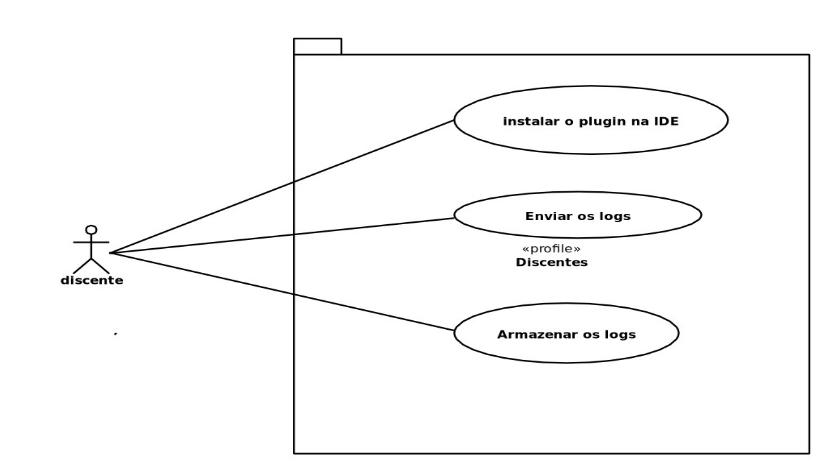
\includegraphics[width=1.1\textwidth]{../figuras/caso-de-uso-discentes.png}
    \caption{Casos de uso da extensão Logado - Visão do Discente}
    \label{fig:casos-uso-discente}
\end{figure}

\begin{figure}[H]
    \centering
    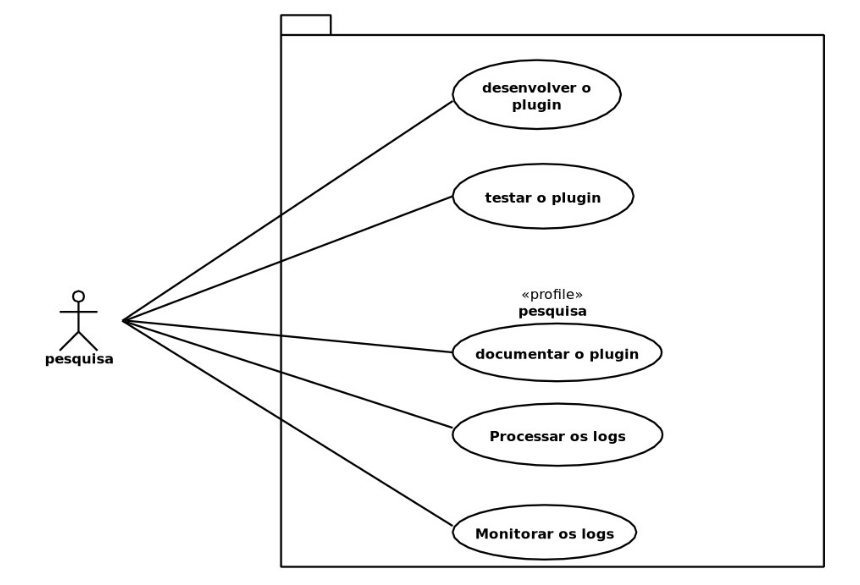
\includegraphics[width=1.1\textwidth]{../figuras/caso-de-uso-pesquisa.png}
    \caption{Casos de uso da extensão Logado - Visão do Pesquisador}
    \label{fig:casos-de-usos-pesquisa}
\end{figure}

A partir dos casos de uso, foram derivados os requisitos formais do sistema:

\paragraph{Requisitos Funcionais}
Os requisitos funcionais definem as funcionalidades que o sistema deve executar. Para o ator \textbf{Discente}, a extensão deve:
\begin{itemize}
    \item \textbf{RF01:} Registrar automaticamente eventos de edição de código (e.g., inserção, deleção de caracteres).
    \item \textbf{RF02:} Capturar eventos de compilação e execução de código, incluindo sucesso ou falha.
    \item \textbf{RF03:} Armazenar localmente os logs com \textit{timestamp} preciso.
    \item \textbf{RF04:} Transmitir os logs anonimizados para um servidor remoto de forma assíncrona.
    \item \textbf{RF05:} Exibir notificações de confirmação de operações para o usuário.
\end{itemize}

Para o ator \textbf{Pesquisador}, a extensão deve:
\begin{itemize}
    \item \textbf{RF06:} Fornecer uma interface de configuração para parametrizar os eventos a serem capturados.
    \item \textbf{RF07:} Gerar identificadores únicos anônimos para cada sessão de uso.
\end{itemize}

\paragraph{Requisitos Não-Funcionais}
Estes requisitos definem os critérios de qualidade para o sistema:
\begin{itemize}
    \item \textbf{RNF01 (Desempenho):} A extensão não deve impactar significativamente o desempenho da IDE. O tempo de resposta deve ser inferior a 100ms para operações de registro.
    \item \textbf{RNF02 (Usabilidade):} A instalação e o uso devem ser simples, não requerendo configuração complexa por parte do discente.
    \item \textbf{RNF03 (Confiabilidade):} A extensão deve garantir a persistência dos logs mesmo em caso de fechamento inesperado da IDE.
    \item \textbf{RNF04 (Segurança e Privacidade):} Todos os dados pessoais devem ser anonimizados antes do envio ao servidor, conforme a LGPD.
\end{itemize}

\paragraph{Desenvolvimento do Artefato}
Desenvolvimento da extensão LOGADO para Visual Studio Code, com funcionalidades de captura de eventos de programação.

\subsubsection{Atividade 4: Demonstração e Avaliação}
\label{subsubsec:demonstracao-avaliacao}

\paragraph{Contexto e Participantes}
Pesquisa será realizada no IFAM Campus Boca do Acre com aproximadamente 80 estudantes do curso técnico em Informática.

\paragraph{Procedimentos de Coleta}
\begin{itemize}
    \item Duração: 3 semanas de aulas práticas
    \item Local: Laboratório de Informática do campus
    \item Ferramenta: Visual Studio Code com extensão LOGADO
    \item Aspectos éticos: Aprovação do Comitê de Ética, TCLE
\end{itemize}

% --- SEÇÃO SOBRE ANÁLISE DE DADOS ---
\section{Plano de Análise de Dados}
\label{sec:analise-dados}

Os dados coletados serão analisados em três etapas:

\subsection{Pré-processamento e Limpeza}\label{subsec:limpeza}
Filtragem e anonimização dos dados, garantindo a privacidade dos participantes.

\subsection{Geração de Métricas Educacionais}\label{subsec:metricas}
Transformação dos logs brutos em indicadores de aprendizagem.

\subsection{Análise Estatística e Identificação de Padrões}\label{subsec:identificacoes-padroes}
Uso de técnicas estatísticas para correlacionar padrões de codificação com desempenho acadêmico.


\section{Cronograma}
\label{sec:cronograma}
Nesta seção é exposto o cronograma previsto para a realização deste trabalho e obtenção de grau de mestre (considerando os requisitos apresentados no Regulamento Interno do Programa de Pós-Graduação em Computação Aplicada (PPGCA) da Universidade Tecnológica Federal do Paraná (UTFPR), campus Curitiba. 
    Na figura \ref{fig:gantt} são listadas as atividades a serem realizadas e os períodos em que estas pretendem ser executadas. As atividades estão organizadas de acordo com as quatro fases detalhadas abaixo, não sendo apresentadas aquelas já finalizadas(e.g.: revisão da literatura - Fase 1; delineamento inicial da abordagem - parte da Fase 2; obtenção dos créditos exigidos pleo PPGCA em disciplinas ou atividades; e aprovação em exame de suficiência em língua inglesa).
    
\begin{figure}[ht]
	\centering
	\begin{ganttchart}[
		vgrid={*{8}{gray!30, dotted}},
		hgrid,
		x unit=1.5cm,
		y unit title=0.7cm,
		y unit chart=0.6cm,
		title/.style={draw=none, fill=none},
		title label font=\bfseries\footnotesize,
		bar/.style={draw=none, fill=blue!40, rounded corners=2pt},
		bar height=0.5,
		bar label font=\scriptsize,
		bar label node/.append style={left=3pt, text width=3cm, align=right},
		milestone/.style={fill=red!70, shape=rectangle},
		milestone label font=\scriptsize\bfseries
		]{1}{8}
		
		% Year and month titles
		\gantttitle{2025}{5} \gantttitle{2026}{3} \\
		\gantttitlelist{8,9,10,11,12}{1} \gantttitlelist{1,2,3}{1} \\
		
		% Activities
		\ganttbar{Qualificação}{1}{3} \\
		\ganttbar{Experimento 1}{4}{5} \\
		\ganttbar{Experimento 2}{5}{6} \\
		\ganttbar{Conclusão da pesquisa}{6}{7}\\
		\ganttbar{Submissão de artigos}{1}{7}\\
		\ganttbar{Escrita da dissertação}{1}{8} \\
		\ganttmilestone{Entrega da dissertação}{7}{8}
		
	\end{ganttchart}
	\caption{Cronograma do trabalho/mestrado}
	\label{fig:gantt}
\end{figure}

Conforme pode ser visualizado na \ref{fig:gantt}, as atividades foram planejadas de modo mensal. Inicialmente, para agosto de 2025 estavam previstas: (1) a qualificação da proposta de dissertação; e (2) a execução da parte da Fase 3, por meio da validação, análise e interpretação dos dados coletados na primeira execução do experimento de avaliação da abordagem (ocorrerá em novembro de 2025). A segunda atividade será finalizada em setembro, sendo seguida pela realização de eventuais ajustes na abordagem (Fase 2), cujo término é previsto para outubro.

Como forma de validação externa da pesquisa, um artigo com o mesmo tema desta dissertação foi submetido à LACLO (Conferência Latinoamericana de Tecnologias de Aprendizagem) e aceito após processo de revisão por pares. Esta aceitação, ocorrida em agosto de 2025, atesta o valor científico do trabalho, que será apresentado no evento em novembro do mesmo ano.

Por sua vez, nos meses de outubro e novembro planeja-se realizar a segunda operação do experimento, bem como análise e interpretação dos dados coletados (seguindo os passos a serem descritos nas subseções 4.2.3 e 4.2.4). Já em dezembro pretende-se concluir a pesquisa (execução das atividades da Fase 4).

 

%fevereiro de 2026 será escrito e submetido artigo relacionado à dissertação em veículo técnico-científico da área, atividade que faz parte da etapa de apresentação e empacotamento do experimento (a ser descrita na subseção 4.2.5).

Acerca da escrita da dissertação, está ocorrerá entre agosto de 2025 e março de 2026. É importante mencionar que a escrita de todos os capítulos pretende ser finalizada ainda em dezembro de 2025, sendo janeiro e fevereiro do ano seguinte destinado a correções e/ou melhorias recomendadas pelos orientadores (antes do envio do documento à banca). Por sua vez, em março serão realizados eventuais ajustes no texto(sugeridos pela banca) após a defesa da dissertação, prevista para o mesmo mês. 

Por fim, após a conclusão das atividades mencionadas acima, ainda em março planeja-se: (1) entregar a dissertação para registro no RIUT; (2) prover feedback dos resultados da pesquisa aos participantes interessados (a indicação de interesse será coletada em campo do Termo de Consentimento Livre e Esclarecido (TCLE), sendo os resultados enviados por e-mail); e (3) elaborar e entregar o relatório final de pesquisa ao CEP da UTFPR, atividade que encerra as atividades previstas para este trabalho. 
